\documentclass[a4paper]{article}

\usepackage[english]{babel}
\usepackage[utf8]{inputenc}
\usepackage{amsmath}
\usepackage{graphicx}
\usepackage[colorinlistoftodos]{todonotes}
\usepackage{hyperref}
\usepackage{ amssymb }
\usepackage[normalem]{ulem}
\usepackage{amsfonts}
\usepackage{amsmath}
\usepackage{graphicx}
\usepackage{float}
\usepackage{bm}
\usepackage{caption}

\usepackage{amsmath,amsfonts,amssymb}




\begin{document}

\noindent \texttt{\emph{Donald Knuth: }Everyday life is like programming, I guess. If you love something you can put beauty into it.}
\ \\

Writing code is important for any probability course. This is because probability is the mathematics of counting, and computers are little more than counting machines. Early in this book, we talked about how most probability questions can be boiled down to enumerating two sets: the set of all possible outcomes and the set of desired outcomes. For example, in our discussion of cards, each problem involved counting the number of hands meeting some set of constraints, and dividing by the total number of possible hands. As we moved into more advanced combinatorics, we retained this reliance on counting. For example, the cookie problem involved counting the number of ways to divide cookies among distinct individuals. Even our discussion of the various random variables governed by probability density functions was motivated by counting. Given a random variable $X$, $P(X=x)$ is simply the number of times $X$ takes on $x$ divided by the total number of trials (as the number of trials approaches infinity). From this, one could even say that the mathematics behind convolutions, moments, and even the Central Limit Theorem are related to counting problems.

The reason we learned so much theory is because counting takes time. As we've seen, counting problems often have to be broken up into cases, subcases, etc.. The cardinality of the set of possible outcomes can be in the millions, or even billions! Even more, the behavior we want often occurs only in the limit. For example, the Central Limit Theorem only applies as the number of i.i.d. summands approaches infinity. It is incredibly time consuming to count such large numbers. By writing simulations with computer code, we can get computers to do all of the heavy lifting for us!

Within the scope of any probabiliy class, computer programming is incredibly useful. We can simulate problems and evaluate event probabilitys to verify our theoretical results. Outside of class, the ability to program is one of {\bf the} core skills of the $21^{st}$ century. If you want a job in tech, finance, buisness, medicine, or any other field, a basic understanding of how to program will prove invaluable.


What if you don't want a technical job? Don't sit here thinking ``this doesn't apply to me" because you WILL interact with computers every day. Programming gives you a deeper of understanding of how computers work. Leveraging computer code will make you better at most modern professions. For example, consider the ability to back up a proposal with a computer simulation. You could even write a program to do your job for you! (\url{http://www.businessinsider.com/computer-program-does-your-job-2013-3}).

As a last aside, learning to program is important because code is the language of the future. Already, many of the highest paying jobs are programming jobs. Computers are becoming increasingly smarter, increasingly nimble, and increasingly capable of taking over most skilled jobs. By the time you are middle aged, computers may have replaced your job (\url{https://www.youtube.com/watch?v=7Pq-S557XQU}). So stay ahead! Learn to code!

\section{Programming Basics}

Learning how to program is a skill that often takes months of practice. That being said, after reading this section you should have a rudimentary grasp of what programming is and the tools reqiured to build software. After reading this chapter, you won't be able to build your own filesystem or web app. However, you should feel comfortable writing simple programs.

I am going to start by discussing a variety of programming languages. I will show you how to execute programs in each language and say a little bit about their pro's and con's. Next, I will cover some basic programming syntax. Each programming language has its own set of rules, but most share common ground. We will focus on that common ground. Next, I will talk about how to break your code into multiple subproblems and tackle each problem with something called {\it methods}. This is a critical programming skill. Last, I will talk about some basic style guidelines that every sensible programmer should follow.

Before we begin, let's think about what a program is. A program is a way to issue instructions to a computer. Human languages are ambiguous and difficult to understand. Code, on the other hand, is unambiguous. Code can be thought of as a list of instructions telling a computer what to do, and each instruction is called a {\it statement} or {\it line of code}. You can write your own programs in any text editor. My favorite is \texttt{emacs}, which you can run by opening the terminal and simply typing in \texttt{emacs}. Some more simple text editors are TextEdit in Mac and WordPad in Windows.

\subsection{Programming Languages}

We have an idea of what a program looks like. It is a collection of statements, or lines of code. We also know that each line of code issues an instruction to the computer, telling it to do something. This is vague on purpose. Each line of code looks different according to the programming language you are coding in. A programming language defines the syntax of each statement, the data types you are allowed to use, and much, much more about what kinds of programs you are and aren't allowed to write.

There are lots of programming languages. You may have heard of some (Java, anyone?), but not all. For example the COW language consists completely of different capitalizations of the word ``moo". Writing your simulations in COW may seem like fun, but it certainly isn't for anyone trying to read your code. In order to make your software more readable, it's a good idea to stick to well-known programming languages.

\begin{figure}
\begin{center}
\scriptsize
\begin{verbatim}
MoO moO MoO mOo MOO OOM MMM moO moO  MMM mOo mOo moO MMM
mOo MMM moO moO  MOO MOo mOo MoO moO moo mOo mOo moo
\end{verbatim}
\normalsize
\caption{\label{fig:cowcode} COW code to generate the Fibbinocci Sequence.}
\end{center}\end{figure}

We are going to focus on five languages: C, Python, Java, Mathematica, and R. We will be paying particular attention to Python as the chapter goes on. C, Python, and Java, are three popular programming languages. Some consider these the ``big three" languages because most modern code is written in one of these languages or a derivative thereof. Mathematica is a language specifically designed for computational problems, and R is an excellent statistical programming package. We will now discuss how to make and run programs in each language, placing special emphasis on C, Python, and Java because those are more helpful languages to know outside of this class.

\begin{figure}
\begin{center}
\scalebox{.5}{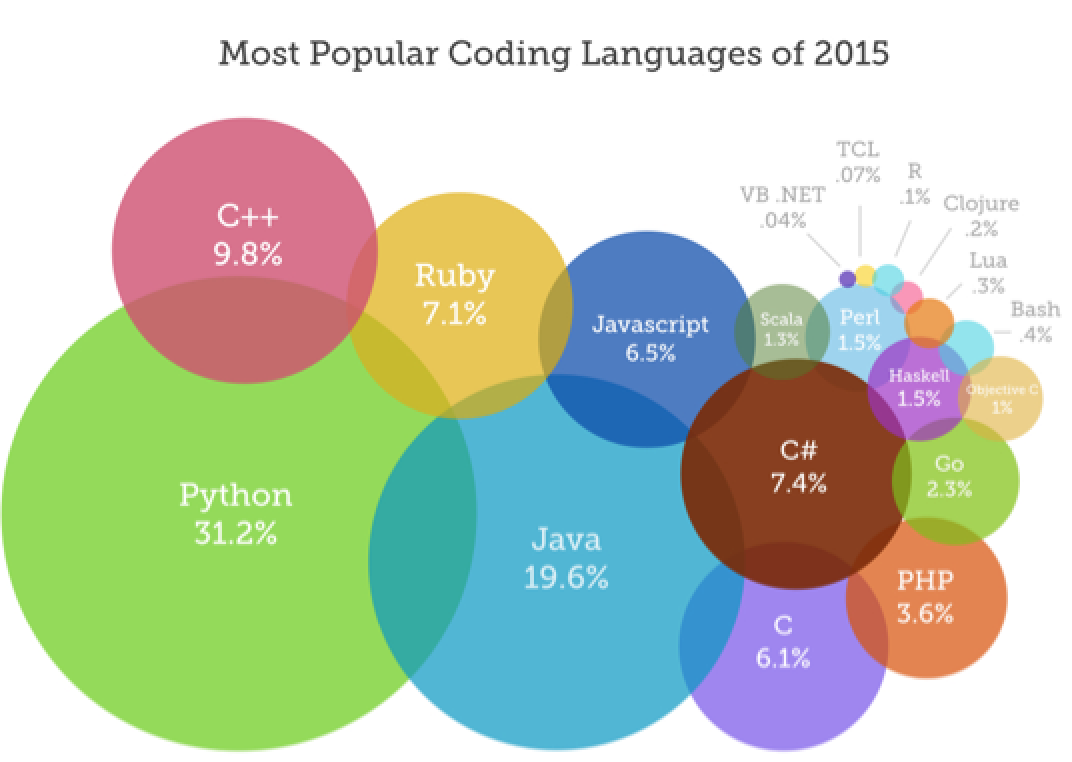
\includegraphics{languagePopularity.eps}}
\caption{\label{fig:languagePopularity} Some of the most popular languages, as determined by coding tests (\url{http://blog.codeeval.com/codeevalblog/2015\#py}). See \url{http://githut.info/} for language statistics on GitHub, a popular online code repository.}
\end{center}\end{figure}

\subsubsection{C}
C is the oldest language of the five - it was developed way back in 1970. C and it's close relative C++ are still some of the most widely used languages in the world. Why? Because they are fast and simple. C lets you work extremely close to the hardware of the computer, which gives programmers more flexibility. On the other hand, this simplicity has a downside - C doesn't come with any extra bells and whistles that other languages benefit from. C doesn't come with any built-in data structures (more on those later) so you have to build them all from scratch.

You \ex can create a C program by ending any raw text file with \texttt{.c}. Type \texttt{gcc -o [executable name] [filename]} into the terminal to compile your file into an executable. Run the executable by entering \texttt{./[executable name]} into bash. See Figure \ref{fig:chello} for a basic C program.


\begin{figure}
\begin{center}
\begin{verbatim}
In the source file (hello.c):
#include <stdio.h>

int main() {
  printf("Hello, world!\n");
  return 0;

}

On the command line:
gcc -o hello hello.c
./hello
\end{verbatim}
\caption{\label{fig:chello} Creating and running a basic hello world program in C.}
\end{center}\end{figure}


\subsubsection{Python}

Python is a powerful language that is easy to read and write. Many of its advocates argue that it is one of the best languages to start programing in because of the simplicity of its syntax and depth of features. Another plus is that Python is interpreted, not compiled. This means that you can execute Python code line by line without having to compile it into an executable. Most of this chapter will be concerned with Python because it's so easy to learn.

You \ex can create a Python program by ending a text file with \texttt{.py}. Enter \texttt{python [filename]} into bash to run the program. You can also open a line-by-line Python interpreter in the terminal window by entering \texttt{python} into bash. This will let you test out code on a per-statement basis. See Figure \ref{fig:phello} for a basic Python program.

\begin{figure}
\begin{center}
\begin{verbatim}
In the source file (hello.py):
print "Hello, world!"

On the command line:
python hello.py
\end{verbatim}
\caption{\label{fig:phello} Creating and running a basic hello world program in Python.}
\end{center}\end{figure}


\subsubsection{Java}
Java is like the WallMart of programming languages. It's big, corporate, and you can find it everywhere. It's one of the most popular programming languages and has strong networking features. Most introductory courses in programming are taught in Java.

You \ex can create a Java program with the \texttt{.java} file extension, compile Java code with \texttt{javac [filename]}, then run your executable with \texttt{java [filename]}. See Figure \ref{fig:jhello} for a basic Java program.

\begin{figure}
\begin{center}
\begin{verbatim}
In the source file (hello.java):
public class hello {
    public static void main(String [] args) {
        System.out.println("Hello, World!");
    }
}

On the command line:
javac hello.java
java hello
\end{verbatim}
\caption{\label{fig:jhello} Creating and running a basic hello world program in Python.}
\end{center}\end{figure}



\subsubsection{R}
R is a statistical package designed specifically for data analysis. Because it is a specialized language, it is better at some things than others. It is good at number crunching, matrix manipulations, and statistical analysis. It is not good for pretty much anything else. Like Python, R is an interpreted language. This means that you can play around with the code one line at a time.

It is best to code in R through an IDE (Integrated Development Environment). The best R IDE is Rstudio (\url{http://www.rstudio.com/}). It is free, and will walk you through all the steps needed to install R and Rstudio.

\subsubsection{Mathematica}
Mathematica, like R, is a specialized language. While R is a statistical package for data analysis, Mathematica is a piece of exploratory software for engineering and scientific computing. Like R, Mathematica is best run in an IDE. Unfortunately, Mathematica isn't free. Get it here (\url{http://www.wolfram.com/mathematica/}).

\subsection{Programming Syntax}

Every programming language has different statements. This can make it scary to pick up a new language, but don't be intimidated! Almost every language (including Java, Python, and C) shares a core set of concepts. Knowing how to use these concepts appropriately is what programming really is. The idiosyncrasies of each languagne are just fluff. Google can be your best friend. If you want your code to perform a specific concept but don't know the right syntactic sugar, just Google it! Nobody expects you to memorize every possible command in every possible language. It's better to know the range of tools that are available to you and when it is appropriate to use each of them.

Here are five core concepts that every programmer should know about. Each one is implemented differently in various languages, but the idea is the same. Many of these concepts are simple logical statements or ideas borrowed from mathematics. Taken individually, each is surprisingly simple. Taken together, these concepts let you write a program as complex as Microsoft Word, or IOS.

\subsubsection{1) Variables}

Variables in code are the same as variables in mathematics. A variable is a named storage location where the computer keeps data. This data is often structured into a {\it type}. Types let the computer know what kind of data is held within the associated variable. Example types include \texttt{int} for integers, \texttt{float} for decimals, \texttt{boolean} for truth variables, and \texttt{string} for text. It's important to note that while the variables in math could be irrational, programming variables are constrained by the limits imposed by computer memory. In most systems, \texttt{int}'s can only range between $+/- 2^{31} - 1$, \texttt{float}s can only represent 7 or 8 decimal places, and \texttt{string} size is limited by the amount of memory a computer system has. Note that all of these constraints can be bypassed with more advanced programming techniques, but it is important to know the basic limitations of standard types.

Here's \ex a few examples of instantiating variables. Type-setting in Python is dynamic, so you don't need to worry about declaring the type of a variable. Thus, creating a new variable in Python is extremely easy. In Java and C, you have to tell the computer what the type of a variable is going to be. This is easy - all you have to do is put the name of the type before the variable name the first time you mention a variable. Note that in Java and C it is also possible to {\it initialize} variables. When you initialize a variable, you are simply letting the computer know that this variable exists without giving it a value. Here are some examples of instantiation and initalization in Python and Java (the syntax for instantiation and initilization in Java is almost identical to that of C).

Python
\begin{verbatim}
# instantiating an int
num = 1
# instantiating a float
decimal = 1.1
# instantiating a string
hello = "hello"
\end{verbatim}

Java:
\begin{verbatim}
// instantiating an int
int num = 1;
// initializing an int
int num_novalue;
// initializing a float
float decimal_novalue;
// instantiating a string
string message = "hello world!";
\end{verbatim}

One \info last note before we leave this introduction to variables. It is possible to change the type of a variable through a technique called {\it casting}. Note that casting a \texttt{float} to an \texttt{int} results in the decimal places simply being dropped. This is easiest to show via example (again, C and Java behave similarly when it comes to casting):

Python:
\begin{verbatim}
# instantiate an int and cast it as a float
# note that casted_num will hold 1.0
num = 1
casted_num = float(num)
# instantiate a float and cast it as an int
# note that casted_decimal will hold 2
decimal = 2.5
casted_decimal = int(decimal)
\end{verbatim}

C:
\begin{verbatim}
int num = 1;
float casted_num = (float)num;
float decimal = 2.5;
int casted_decimal = (int)decimal;
\end{verbatim}


\subsubsection{2) Operators}

{\it Operators} are inorder syntactic shortcuts for common functions that act on variables. The order of operations in most programming languages closely resembles that of mathematics. You’re probability familiar with arithmetic operators. They are \texttt{+}, \texttt{-}, \texttt{*}, and \texttt{/}. It is important to know that operands must be of the same type (except in Python). For example, it is bad to try \texttt{A / B} where \texttt{A} is a decimal and \texttt{B} is an integer. If you want to perform decimal division, make sure to cast both the numerator and denominator as \texttt{floats}.

Some other important operators are logical operators. \texttt{\&\&} (and) is true if both operands are true and false otherwise. \texttt{||} (or) is true if either operand is true and false otherwise. \texttt{!} (not) takes the boolean compliment of its operand. Inequality operators (\texttt{<}, \texttt{<=}, \texttt{>}, \texttt{>=}) behave as expected.

A \info new class of operators you may not have seen are bitwise operators. Recall that all numbers are stored in binary on computer systems. \texttt{\&} returns the {\it bitwise and} of two numbers. This is 1 where both digits are 1. \texttt{|} returns the {\it bitwise or}. This is 1 where either digit is 1. \texttt{\~} returns the {\it bitwise complement} of its operand. \texttt{\^} returns the {\it bitwise exclusive-o}r of its operands: it returns 1 where only one of its operands is 1. \texttt{<<} and \texttt{>>} are {\it bit shifters}. They shift the bits of their operands left and right by 1, respectively.

The last group of operators I will discuss are {\it equality} and {\it assignment}. It is important to remember that these are {\bf not the same}. \texttt{=} assigns the value of the right-hand side to the variable on the left hand side. \texttt{==}, on the other hand, tests whether two variables (e.g. \texttt{int}s) are equal. \texttt{string} and \texttt{float} comparison are performed differently because of how they are stored by the computer. For \texttt{string}s, many languages provide built-in functions for equality checking. For \texttt{float}s, use a small delta and see whether the difference between each operand is less than delta.

Many operands can be grouped together. Let's say that we have two integer variables \texttt{A} and \texttt{B}. \texttt{A += B} adds \texttt{B} to \texttt{A} and places the result back in \texttt{A}. \texttt{A >>= B} shifts \texttt{A} to the right by \texttt{B} and places the result in \texttt{A}. \texttt{A++} increments \texttt{A} by 1, and \texttt{A--} decriments \texttt{A} by 1. Note that Python does not support \texttt{++} and \texttt{--}.

Last, grouping operators are used to tighten programming scope and set computation priorities. Parentheses \texttt{()} are the only ones you need to know about, and they define the order of operations the same way as in mathematics.

Let's \ex  do some examples! Since all of the operations behave the same in Python, Java, and C, we will perform these computations in Python.

\begin{verbatim}
# initialize two int variables A and B
A = 5
B = 6
# initialize a new variable, C, which holds 11
C = A + B
# C now holds 16
C += A
# C now holds 32
C <<= 1
\end{verbatim}

\subsubsection{3) Control Structures}

Up to this point, we have variables and a few operations defined on our variables. We have no way to get the computer to make decisions. Control structures are just what we need. These are blocks of code that augment the flow of computation. They analyze one or more variables and allow the computer to make a decision as to what code it will execute next based on these variables. There are many fancy control structures, but I'm just going to show you the basics.

\begin{itemize}
\item {\bf Choice.} This is a way to get the computer to choose one portion of code. \texttt{if} statements are the easiest way to create choice. \texttt{if} statements can be paired with an \texttt{else} statement or an \texttt{else if} statement (or, in Python, \texttt{elif}), which execute only when the initial \texttt{if} condition failed. Here's a few examples of if statements in Python and Java (again, Java and C are very similar in this respect).

Python:
\begin{verbatim}
# initialize variable a to 5
a = 5
# if a is less than 4, set a to 1 (this is not taken2)
if (a < 4):
  a -= 4
# if a is 1, subtract 3 from a
if (a == 1):
  a -= 3
# else if a is 5, subtract 2 from a (this branch is taken)
elif (a == 5):
  a -= 2
# as a base case set a to 0
else:
  a = 0
\end{verbatim}

Java (same code):
\begin{verbatim}
int a = 5;
if (a < 4) {
  a -= 4;
}
if (a == 1) {
  a -= 3;
} else if (a == 5) {
  a -= 2;
} else {
  a = 0;
}
\end{verbatim}



\item {\bf Loops.} A loop is a block of statements which are executed several times in succession. Often, a variable called an {\it index} is updated on each iteration to track your progress. There are two types of loops that you should know about: \texttt{for} loops and \texttt{while} loops. \texttt{for} loops should be used when you know the desired number of iterations, and \texttt{while} loops should be used when you are simply iterating until some condition has been met. Here are some examples of the two looping structures in Python and Java.

Python:
\begin{verbatim}
# print 0 through 9
for i in range(10):
  print i
# print 0 through 9 using a while loop
i = 0
while (i < 10):
  print i
\end{verbatim}

Java:
\begin{verbatim}
for (int i = 0; i < 10; i++) {
  System.out.println(i);
}
int i = 0;
while (i < 10) {
  System.out.println(i);
}
\end{verbatim}

\end{itemize}

In these examples, the index variable was \texttt{i}.

\subsubsection{4) Data Structures}

Imagine you are writing a program to keep track of your address book. You may have hundreds of phone numbers, names, notes, and addresses. It may seem daunting to create a unique variable to store every piece of data you wish to keep track of. First, the sheer amount of code you would have to write would be staggering. Second, your code would be inflexible. If you wanted to add a new contact to your list, you would have to manually edit your code and create a new custom variable.

We need a better way to store data in bulk. Fortunately, there is a right way to store and organize data with something called {\it data structures}. Data structures are themselves variables, so you can refer to them by name and type. However, since data structures are more complex than simple \texttt{int}s or \texttt{float}s, most data structures have a unique set of operations. There are many data structures, but we will only describe three of the most basic. These are arrays, hash tables, and objects.

\begin{itemize}

\item {\bf Arrays.} Almost  every programming language has some kind of array structure. Arrays are linear collection of elements, each identified by an index. It is important to note that array indexing always begins at 0. Thus, accessing the $1^{st}$ element of array \texttt{A} would be performed with \texttt{A[0]}.

Many of the details governing arrays are language-specific. Some languages require you to tell the computer how long an array is when you create it. Other languages let you create an empty array and fill it on the fly. The elements in an array could be of the same type (for example, an array of \texttt{int}s) or of different types (an array of \texttt{int}s and \texttt{string}s) depending on the language you are coding in. Java, for example, only supports single-type arrays. Python, on the other hand, lets you put whatever you want into an array. Here are some example Python and Java arrays, along with some basic operations you might need.

Python:
\begin{verbatim}
# initialize an empty array
A = []
# instantiate a filled array
B = [1,2,3]
# add an element to A. A is now [4]
A.append(4)
# combine A and B. C is [1,2,3,4]
C = B + A
# change the 1st element of C from 1 to 0
C[0] = 0
# print all of the elements in C
for element in C:
  print element
\end{verbatim}

Java:
\begin{verbatim}
int[] A = new int[1];
int[] B = {1, 2, 3};

A[0] = 4;

int[] C = new int[4];
for (int i = 0; i < 3; i++) {
  C[i] = B[i];
}
C[4] = A[0];

C[0] = 0;

for (int i = 0; i < 4; i++) {
  System.out.println(C);
}
\end{verbatim}

\item{\bf Hashtables.}

\begin{figure}
\begin{center}
\scalebox{.5}{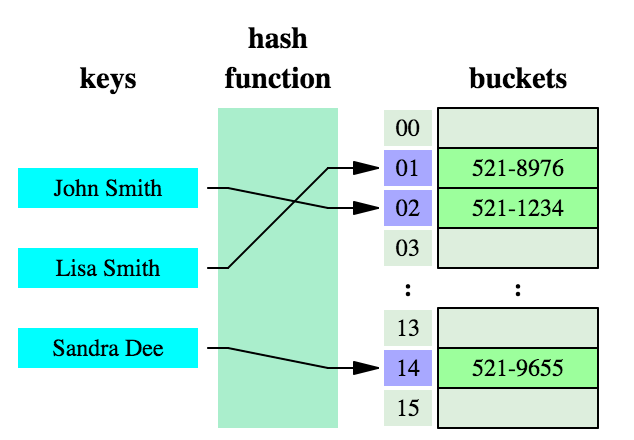
\includegraphics{hashtable.eps}}
\caption{\label{fig:hashtable} Schematic of a hashtable mapping names to phone numbers. \url{http://upload.wikimedia.org/wikipedia/commons/7/7d/Hash_table_3_1_1_0_1_0_0_SP.svg}}
\end{center}\end{figure}

Arrays organize their elements by index. This can be helpful in many applications, but sometimes we may want to organize our data differently. Consider, for example, the address book example from before. What if we want to give our data structure someone's name and receive a phone number? Hash tables are perfect for this! A hash table is essentially a one-to-one mapping between two sets of elements. One set are the {\it keys} and the other are the {\it values}. The mapping function is called a hash function, and there is a lot of interesting mathematics that goes into creating a good hash function. All you need to know, though, is that if you present a hash table with a key, the data structure will return that key's associated value.

Like with arrays, the details surrounding hash tables vary by language. Python has fantastic hashtable support. Python hashtables are called dictionaries. C, on the other hand, has no built in hash table. If you want to use a hash table in C, you'll either need to build one yourself or use an external library (covered later). Java provides native hash table support, but Java hash tables are a little more difficult to use. Because of the ease of use of Python dictionaries, we will only provide examples in Python.

\begin{verbatim}
# initialize an empty dictionary
A = {}
# instantiate a filled dictionary
B = {'example-key': 'example-value', 'key2': 2}

# add a key-value pair
A['key'] = 'value'
A[2] = 5
A[9] = [3, 'hello']

# print 5
print A[2]
# remove the 2:5 mapping from A
del A[2]
\end{verbatim}

\item{\bf Objects.} Objects \info are incredibly useful for software development, but less so for simulation. Lets say that your address book is a little more complicated than simple name-number pairings. Suppose you want to store multiple fields for each entry. In this case, an object may be helpful. An object, or class, is essentially a custom data structure. Objects let you package whatever variables you want into a single entity. Objects also let you define special functions to manipulate their internal data. In the case of our address book, these functions could be editing an entry, adding a new entry, etc. Note that once an object has been created, you can only modify its internal data through these functions. The set of functions that you can use to act on an object is known as the ``interface" of that object.

\end{itemize}


\subsubsection{5) Libraries}
Like mathematicians, programmers are lazy. Good code makes use of other people's code. Libraries are how code sharing happens. Libraries are pre-written collections of code that you can easily bring into your own programs. For example, say you want to read in the text from a file. This is hard to program. Chances are, a far better programmer than you wrote the code for reading text and placed it in a library (as a matter of fact, this library is called \texttt{sys} in Python and \texttt{java.util} in Java).

As   a beginning programmer (especially one concerned with simulation), you should take advantage of libraries whenever you can. It can be hard to guess what you should implement and what can be outsourced to an external library. A good rule of thumb is to give libraries the benefit of the doubt. If you want to do something that seems hard to code (hint: generating random numbers), Google for an associated library.

Two important Python libraries that you should be aware of are \texttt{random} and \texttt{math}. These packages let you generate random numbers and perform common mathematical functions (like log, exponents, square roots, etc.). See section 24.2 to see these libraries in action.


\subsection{Code Organization}
Lets say you want to simulate a game of poker. You will have to draw a random hand of cards from the deck many times. Each draw will be performed with the same code. Rather than replicating your code many times, wouldn’t it be nice if there was a single custom function you could call (say, \texttt{drawHand()}) that would give you a random hand every time? You can make one!

A method is a block of statements that are packaged together as a single unit. Methods may also be called functions, routines, procedures, or subroutines based on context and language. When you ``call" a method, the computer jumps to the code inside that method. After it has finished executing the code within the method, the computer resumes execution right after the point where the method was called. Like mathematical functions, you can give methods arguments (called {\it parameters}) to operate on. When the method is called, it has access to whatever parameters the user chose to pass. However, methods cannot access variables outside of their scope (variables belonging to other parts of the program that were not passed). Identifying which parts of a program should be packaged up into methods is hard. A good strategy is to break a problem into a series of smaller parts, placing each part in its own method.

It \ex is important to know that the framework of a program exists in something called a {\it main method}. This is the core of your program and the place where all other methods are called from. Some languages, like Java and C, have an explicitly defined main method. Scripting languages like Python, R, and Mathematica have no main method. Instead, you can think of their main methods as all of the code that exists outside of a method. Here are some examples of methods in Python and C.

Python:
\begin{verbatim}
def add(a, b):
  return a + b

# main program body starts here
a = 5
b = 1
# c gets 6
c = add(a, b)
\end{verbatim}
C:
\begin{verbatim}
int add(int a, int b) {
  return a + b;
}
int a = 5;
int b = 1;
int c = add(a, b);
\end{verbatim}


\subsection{Best Coding Practices}

At this point, you have all the tools you need to code basic simulations. You know how to create variables of different types. You know how to modify these variables with operations, and how to create complex behavior with iteration and control statements. You even know how to create your own functions and methods as well as using other peoples methods (through libraries). You have one more thing to learn before seeing some heavy duty examples. When it comes to programming, just knowing the tools isn't enough. You have to know what situations are best for each tool. You have to know how to write beautiful code.

So what's ``beautiful code"? Beautiful code works well and is easy to understand. It also follows a few tacit laws of programming. A good program should meet its specification. In other words, a good program performs the task you think it performs, and it performs that task correctly. The code in a good program is efficient. It can be hard to know what commands are easy for a computer to execute and what commands waste time, but the examples in section (2) should give you a little insight into what efficiency looks like. Good code is also easy to maintain. Maintainable code is easy to read and modify. Imagine someone else has to read your code and understand what it does (this will probably be the case!). You want to make their job as easy as possible. So write the clearest, most straightforward code you can without loosing out on correctness. A good strategy to making code readable is to make heavy use of methods. By breaking problems up into smaller peices. Creating independent, modular chunks (and labeling each chunk by placing it into a method), will make the structure of your code shine through the syntax.

To give you a push in the right direction, here are some tips. You may think this section is optional and skip over it. This is not the case. This may be the most important section of the chapter so far. When you write code, you are writing code for other people. A computer may be able to understand your code, but if your boss, professor, or TA can't than it might as well not work at all. The best code makes its functionality self-evident. 

\begin{itemize}
\item {\bf Comment your code.} Every programming language supports comments. Comments are meant for people; they will not be executed by the computer. You've already seen comments in many of our code examples. In Python, a line of comments begins with \texttt{\#}. In Java and C, comments begin with \texttt{//}. What are good things to include in a comment? A good rule of thumb for beginning programmers is that you can never comment too much. At the very least, place a comment above each method to explain what the method is supposed to do. Additionally, comment any lines of code that might be hard to understand.

\item {\bf Consistent spacing.} Each time you enter a new pair of brackets, your code should be tabbed-in. Most IDE's will do this automatically for you, and all of the examples so far have followed this standard. Other than tabs, there are many ways of indenting and organizing your code. I prefer the PEAR coding standards (\url{http://pear.php.net/manual/en/standards.php}), and these standards are exhibited in all of the example code in this chapter. Another spacing strategy is grouping your code. More often than not, a process you want to code will require many statements. It is a good idea to separate these subtasks from each other by putting a space in between each section. There's an added benefit to code grouping: before each block of code is a great place for a comment!

\item   {\bf Reduce redundancy.} Programs are designed to automate repetitive procedures. This principle should extend to the program itself. If you have to type the same line of code twice, this might be a sign that you could improve the structure of your program. Often, repeated blocks of code can be brought out into a method.

\item   {\bf Avoid deep nesting.} Nested code is layered code. This definition is purposefully vague because nesting can spring up in many situations. The two most frequent cases of nested code are nested control structures and nested method calls:

Here's \ex some deeply nested Python code:
\begin{verbatim}
n = 3
if (n > 1):
  if (n < 10):
    n = 0
\end{verbatim}
This could be written more clearly as
\begin{verbatim}
n = 3
if (n > 1 and n < 10):
  n = 0
\end{verbatim}

Deeply nested programs are hard to read and inefficient. If your program has 3 or more nested layers, it is generally a good idea to take a step back and reconsider its code. See if there is a better way to structure your code. Try to unspool all of those \texttt{if} statements.

\item {\bf Consistent variable naming.} There are two naming paradigms. In \\{\it camelCase}, the first letter of each word is capitalized except for the first. In \\{\it underscore$\_$names} each word is separated by an underscore. There is no ``best" naming scheme. The creators of some languages put out official naming guidelines, but at the end of the day these guidelines are nothing more than suggestions. Pick whichever paradigm suits you, but {\bf STAY BY IT}. The important thing is to pick a scheme and stick by it. Doing otherwise makes your code confusing and difficult to read.
\end{itemize}

\section{Example: Coding the Central Limit Theorem}
\subsection{Motivation}
By this point, we have a rudimentary grasp of some basic programming syntax. We know about methods, variables, loops, if statements, and a few different languages to implement these concepts in. We also know some good coding practices to help steer us towards more elegant code. This is all well and good, but half of the challenge of programming is knowing {\it what} to code, not just {\it how} to code. It can be hard to look at a problem and translate it into computer-readable code. Often, the best way to develop the intuition for this is by example. In this section, we are going to walk through one such example.

The Central Limit Theorem is one of the greatest results in probability. In this section, we will simulate it. First, we will create several random number generators from scratch. We will then create a variable to represent the sum of exponential random variables, and show how the distribution of that sum approaches a Gaussian in the limit. I will walk you through the coding process in two languages (C and Python) one step at a time and show all of the thinking that goes on behind the scenes. The aim of reading this section is to develop your programmatic intuition.



\subsection{Uniform Random Number Generator}
We begin by coding a uniform random number generator from scratch. Recall from section 13.1.4 that if we had a perfectly fair coin, we could flip it $n$ times and let $a_i = 1$ if the $i^{th}$ toss is a head and 0 if it's a tail. We then form the number
\[\frac{a_1}{2}+\frac{a_2}{2^2}+\frac{a_3}{2^3}+\cdot\cdot\cdot+\frac{a_n}{2^n} \in [0,1]\]

So how should we code this? First, we note that there is a repeated process going on. Each of the $a_i$'s is determined by a coin flip. Each coin flip is no different than another. It sounds like coin flips are a good thing to put in a method! We also note that the act of drawing a number from the uniform distribution is also a stand-alone process, so this should be a method as well.

Let's begin to think about how we would go about implementing these two methods. We will start with the coin flip method, because (a) it's simpler and (b) the uniform-drawing method will depend on it. We don't know how to simulate coin flipping, so we will use a package. C has the \texttt{rand()} function from the \texttt{stdlib.h} library. This returns a random number between 0 and something very large. We'll just mod that by 2 to get a 0 or 1. Python has the built-in \texttt{random()} function from the \texttt{math} library. This returns a random number between 0 and 1. Though this is essentially a uniform random variable, remember that the important stuff in this section is the code were writing, not the result itself. Once we draw our random number in Python, let's test whether it is less than 0.5 to model a coin flip. As of now, our code looks like this:

Python:
\begin{verbatim}
from random import random

def coin_flip():
    if random() < 0.5:
        return 1.0
    else:
        return 0.0
\end{verbatim}

C:
\begin{verbatim}
#include <stdlib.h>

int coin_flip() {
  return rand() % 2;
}
\end{verbatim}

On to defining our \texttt{uniform()} method! The idea is the same regardless of language. We want $n$ terms in our summation, so we should have a loop that iterates $n$ times before completing. The functionality of each iteration should be the same as computing a single term in the series we're emulating. On iteration $i$ we flip a coin, divide the result by $2^i$, then add this term into the sum. This is implemented below:

Python:
\begin{verbatim}
def uniform(n):
    denominator = 2
    sum = 0.0
    for i in range(n):
        sum += (coinFlip() / denominator)
        denominator <<= 1
    return sum
\end{verbatim}


C:
\begin{verbatim}
// c floats are LIMITED to 2^31 - 1
float uniform() {
  int i;
  int denominator = 2;
  float sum = 0.0;
  for (i = 0; i < 31; i++) {
    sum += coinFlip() / (float)denominator;
    denominator <<= 1;
  }
  return sum;
}
\end{verbatim}

There's a lot going on here. Lets take a moment and try to parse some of it out. First, notice the difference in looping structure between the two languages, and the lack of braces \& semicolons in the Python code. Notice how both the sum and denominator variables are initialized to their starting values. \texttt{sum} is initialized to 0.0, not 0, because it is going to hold decimal numbers. Adding the .0 lets Python know that \texttt{sum} will hold decimals. Putting \texttt{float} before the variable name does the same thing in C. Next, notice that the for loop in the C code is bounded by 31, not $n$. This is because the percision of the \texttt{float} datatype is limited in C. Last, notice that the bits of the denominator were shifted left by 1 instead of squaring. Recall that integers are stored in base 2 in the computer. So the \texttt{<<= 1} operation is the same thing as squaring. I chose to take this less intuitive approach because it is fast and efficient. Computers represent numbers in binary, so bitwise operations are the fastest. Using some rudimentary tests, bit-shifting the denominator allows a 2012 Macbook Pro to generate random numbers \%412 faster when $n = 1000$.

\subsection{Exponential Random Number Generator}
We now turn to the task of coding an exponential random number generator. This will make use of our uniform random number generator. Recall from 13.2.3 that, given a uniformly distributed variable $y$, we may draw numbers from an exponential distirbution governed by $\lambda$ with
\[x = -\lambda \textrm{log}(1-y)\]
Why? This function is the inverse of $F_X(x) = y$. Thus, we are picking a random $y$ value and feeding it backwards through the CDF of the exponential distribution. This translates our $y$ value into an exponentially distributed $x$.

Now that we know the mathematics behind generating random numbers exponentially, let's think about how to translate these ideas into code. We want to draw $y$ from the uniform distribution. This is easy! We can just call our trusty \texttt{uniform()} method from 24.2.2. It looks like we also want to take a logarithm. This is not an easy task to code, so let's use a library to help us out. The Python \texttt{math} library and the C \texttt{math.h} library both have built-in log functions. There's one more thing to think about before we start writing some code. We parameterize the formula with a $\lambda$ of our own choosing. This means that our \texttt{exponential()} method should take \texttt{lambda} as a parameter. Now that we've thought about all of the variables, parameters, and method calls that need to happen in this method, everything else is going to be an easy multiplication or subtraction. We're ready to write some code!

Python:
\begin{verbatim}
from math import log

def exponential(lambda):
    y = uniform()
    return -lambda * log(1 - y)

\end{verbatim}


C:
\begin{verbatim}
#include <math.h>

float exponential(int lambda) {
  float y = uniform();
  return -lambda * log(1 - y);
}
\end{verbatim}

This code is pretty self-explanatory. Because Python has dynamic typing, we don't need to tell the computer whether $\lambda$ or \texttt{y} are reals or integers. C, on the other hand, must be explicitly typed. \texttt{float} is used in variable declarations when we want that variable to store decimals. Since $\lambda$ is an integer, its type is \texttt{int}.

\subsection{Gaussian Random Number Generators}

On to the Central Limit Theorem! We are going to simulate the CLT with our \texttt{exponential()} method. If we let $x_i$ be exponentially distributed, $X = \sum_{i=0}^n x_i$ should become normally distributed as $n$ approaches $\infty$. In order to simulate this theoretical result, we will compute the sum of exponentially distributed summands and observe whether the distribution of these values becomes bell-shaped as the number of summands increases.

Let's get to work. This method should take $n$ as a parameter because the Gaussian variable we want to return is a function of the number of exponential summands. First, we want to create a variable to hold the value of our ever-increasing sum. Next, we want to define a loop that iterates $n$ times. Since we know the number of iterations, we should use a \texttt{for} loop. Each iteration should draw a number from the exponential distribution (let's use our \texttt{exponential()} method from before) and add it into our accumulator variable. At the end of the day, the accumulator is returned. Here's the code:

Python:
\begin{verbatim}
def gaussian_CLT(n):
    x = 0.0
    for _ in range(n):
        x += exponential()
    return x
\end{verbatim}


C:
\begin{verbatim}
float gaussian_CLT(int n) {
  float x = 0.0;
  int i;
  for (i = 0; i < n; i++) {
    x += exponential(2);
  }
  return x;
}
\end{verbatim}

That wasn't too bad, was it?


\subsection{Simulating the CLT}
We're finally here! It's time to see whether all of the theory checks out, and the sum of exponentially distributed random variables is itself normally distributed in the simulated limit. We have a Gaussian random number generator based on the sum of exponentially distributed random variables. The easiest way to see whether this generator is actually Gaussian is by plotting it. Before plotting a histogram of our data, though, we are going to normalize so that the resulting plot is normally distributed ($\mu = 0$ and $\sigma = 1$). Recall that creating a normalized variable $X'$ from $X$ involves the following computation:
\[ X' = \frac{X - \mu}{\sigma}\]

So how on earth are we going to do this programmatically? We begin like we always do, by breaking up the problem into smaller parts. We will have to compute $\mu$, the mean, and $\sigma$, the standard deviation of our data. But what is ``our data"? The best representation would be an array, because we need to store each datum in an easily accessable location. Note that C does not support arrays. You will need to implement them from scratch, which is outside the scope of this chapter. Because of this, we're going to leave our dear friend C at this point and proceed with Python.

Let's recap. At this point, we know that we will have to draw $n$ numbers from our \texttt{gaussian\_CLT} method and place them into an array. We will then use this array to compute the mean and standard deviation of the data. Last, we will normalize each element of the array. Now, if we plot a histogram of the data held in this array, it should be a normally distributed bell curve. Because computing the mean, standard deviation, normalization, and plotting are all seperate functions, each of these code blocks should be exported to a seperate method. The driver code, on the other hand, will be the framework of our program so it can be written as our main method and placed at the bottom of our code.

Let's begin with computing the mean. Given an array, we want to sum up all of the elements in that array and divide by the number of items (its length). Fortunately, Python gives us the built-in \texttt{sum()} and \texttt{len()} methods, which compute the sum and length of arrays, respectively. This makes our code easy:

\begin{verbatim}
def mean(array):
    return sum(array) / float(len(array))
\end{verbatim}

The reason we passed \texttt{len(array)} to \texttt{float()} (we could have also said ``casted into a float") is because Python needs the denominator of a fraction to be a decimal if the quotient is to be a decimal. Calling \texttt{float()} performs this cast.

Now on to the standard deviation. Recall that the definition of $\sigma$ is
\[\sigma\ =\ \sqrt{\frac{1}{n}\sum_{i=1}^n (x_i - \mu)^2}.\]

Since \task we will need to access each element of data, we will need the data array passed as a parameter to our standard deviation method. At this point, you have seen every operation we will have to perform. We will use the \texttt{sqrt} method from the \texttt{math} library to compute square roots. I am going to start removing the training wheels and give you the code right off the bat. Take a moment and try to write this method yourself. Really. Here's a hint: you should use a \texttt{for} loop. How did it go? In any case, here's the code.

\begin{verbatim}
def std_dev(array):
    n = float(len(array))
    mu = mean(array)
    ss = 0

    # compute the sum of squares
    for x in array:
        ss += ( (x - mu) * (x - mu) )

    return sqrt(ss / n)
\end{verbatim}

Note that we avoided using our bit-shifting trick from before because that only works for integers, and \texttt{x - mu} is a \texttt{float}.

On to data normalization! This method should take the data array as a parameter and return a new, normalized dataset. All it has to do is compute the mean, standard deviation, then loop through the data array setting each $x_i$ to $x_i'$. The code is as follows:

\begin{verbatim}
def normalize(array):
    mu = mean(array)
    sigma = std_dev(array)

    for i in range(len(array)):
        array[i] = (array[i] - mu) / sigma

    return array
\end{verbatim}

On to the driver code, or ``main method". We want to draw $n$ numbers from the exponential distribution, placing each element into an array. We then want to plot a histogram of the normalized data. We will use the family of \texttt{plt} functions from the \texttt{matplotlib.pyplot} library to create these histograms. It would be nice if users could enter their desired value for $n$ when the run the program. We can do this by using the \texttt{argv} array in the \texttt{sys} package. Our code is as follows:

\begin{verbatim}
import matplotlib.pyplot as plt
from sys import argv

def hist(x, xlab="Number", title="Histogram", ylab = 'Frequency'):
    plt.hist(x, bins=25, color='blue')
    plt.ylabel(ylab)
    plt.xlabel(xlab)
    plt.title(title)
    plt.show()

N = int(argv[1])

data = []
for _ in range(N):
  data.append(gaussian_CLT(100))

hist(normalize(data))
\end{verbatim}

Note that all of the items kept in \texttt{argv[]} are strings, so we need to transorm it into an integer by calling \texttt{int()}. We arbitrarally chose 100 for the number of exponential summands. Also note the underscore in the declaration of our foor loop. This lets Python know that we don't need a variable to keep track of each iteration and that we just want to execute the statements in the body of the loop $n$ times.

Phew!! We're finally done! Let's look at out entire program one more time, then run it and see if all of this work paid off. Here's the code:
\scriptsize
\begin{verbatim}
import matplotlib.pyplot as plt
from random import random
from math import log, sqrt
from sys import argv


def hist(x, xlab="Number", title="Histogram", ylab = 'Frequency'):
    plt.hist(x, bins=25, color='blue')
    plt.ylabel(ylab)
    plt.xlabel(xlab)
    plt.title(title)
    plt.show()

def coin_flip(p = 0.5):
    if random() < p:
        return 1.0
    else:
        return 0.0

def uniform(n = 30):
    denominator = 2
    sum = 0.0
    for i in range(n):
        sum += (coin_flip() / denominator)
        denominator <<= 1
    return sum

def exponential(lmbda = 2):
    y = uniform()
    return -lmbda * log(1 - y)

def gaussian(mean = 0, stdDev = 1):
    d = 1.0
    while (d >= 1.0 or d == 0):
        x = uniform() * 2 - 1
        y = uniform() * 2 - 1
        d = x * x + y * y

    d = sqrt( (-2.0 * log(d)) / d )

    return mean + std_dev * d * x

def gaussian_CLT(n):
    x = 0.0
    for _ in range(n):
        x += exponential()

    return x

def mean(array):
    return sum(array) / float(len(array))

def std_dev(array):
    n = float(len(array))
    mu = mean(array)
    ss = 0
    for x in array:
        ss += ((x - mu) * (x - mu))
    return sqrt(ss / n)

def normalize(array):
    mu = mean(array)
    sigma = std_dev(array)

    for i in range(len(array)):
        array[i] = (array[i] - mu) / sigma

    return array


N = int(argv[1])

data = []
for _ in range(N):
    data.append(gaussian_CLT(100))

hist(normalize(data))
\end{verbatim}
\normalsize

Notice that all of our library references are at the top, all of our method definitions are in the body, and our driver code is at the end of our program. Let's run it!

\begin{figure}
\begin{center}
\scalebox{.5}{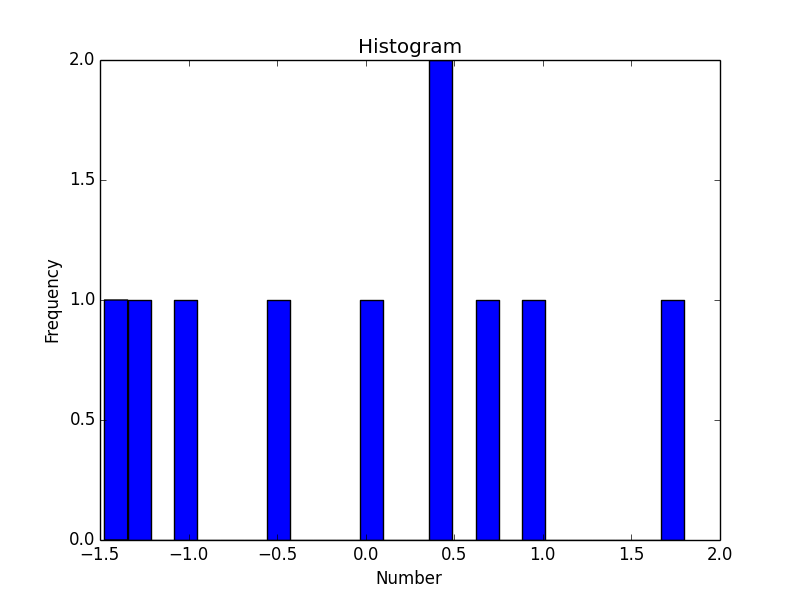
\includegraphics{10.eps}}
\caption{This was created with $n=10$, using the line \texttt{python code.py 10}. It looks like the $n$ we chose is too small. Let's bump it up a few orders of magnitude.}
\end{center}\end{figure}


\begin{figure}
\begin{center}
\scalebox{.5}{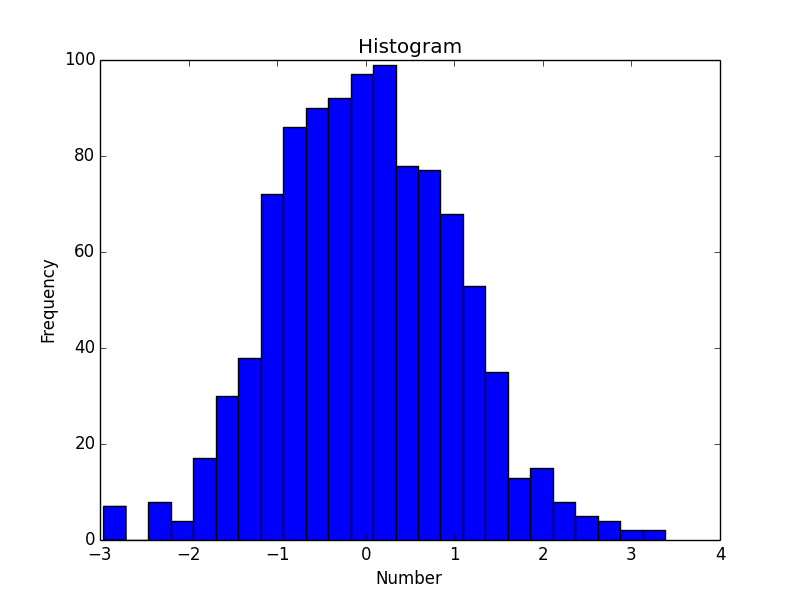
\includegraphics{1000.eps}}
\caption{$n = 1000$, \texttt{python code.py 1000}. Better...}
\end{center}\end{figure}


\begin{figure}
\begin{center}
\scalebox{.5}{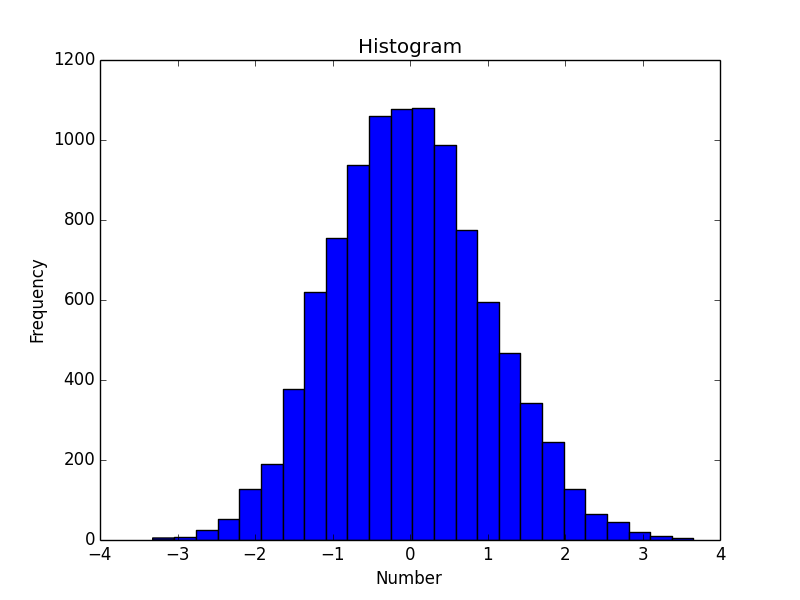
\includegraphics{10000.eps}}
\caption{$n = 10000$, \texttt{python code.py 100000}. Looks pretty good! I guess the CLT is true after all!}
\end{center}\end{figure}

If you wish to download this code and try running it yourself, visit \url{https://github.com/rpryzant93/CLT_simulator/blob/master/CLT_simulator.py}.

\section{Summary}

Teaching people how to code is suprisingly difficult. A complete understanding would require you to take Computer Science classes. Fortunately there's loads of free courses online. Coursera (\url{https://www.coursera.org/course/interactivepython1}), Udacity (\url{https://www.udacity.com/course/intro-to-java-programming--cs046}), and Harvard's CS50 (\url{https://cs50.harvard.edu/}) are all fantastic resources for learning the basics of Computer Science.

This chapter was intended to give you a bare-bones understanding of code so that you are well-equipped to write some basic simulations. We noted that the vast majority of skills you learn in one programming language are transferrable to other languages. We used this observation to learn a few core concepts that are common to all languages. We put all of this into practice by simulating the CLT one step at a time. But remember that learning how to program is like practicing musical scales - it helps you become a better musician, but it's just not the same as playing music. Code is really about solving problems and explaining that solution to a computer. So take your time and play some music. Think before, during, and after you code because a good solution is easier to read and write than a bad one.

\end{document}
